%
%  Chapter:  3 - 135Pr Experimental Methods
%  Modified: 2/16/2015
%  Author:   James Till Matta
%
%%%%%%%%%%%%%%%%%%%%%%%%%%%%%%%%%%%%%%%%%%%%%%%%%%%%%%%%%%

\chapter{EXPERIMENTAL METHODS}
\label{chp:exp-pr}
Across all of experimental physics there is a common theme in the design of an experiment. Finding a way of producing the system to be studied is one part of this theme. The other part is having the equipment to collect the signals necessary to understand what the system is doing. In nuclear physics, the appropriate choice of reaction will create the desired system and the equipment for signal collection will depend greatly on what one wishes to measure or find. This chapter will discuss the reaction, detectors, and techniques used in the examination of transverse wobbling in \pr{}.
\section{Heavy-ion Fusion-evaporation Reaction}
\label{sec:exp-pr-fus-evap}
Across nuclear physics there are vast array of reactions used. Narrowing to in-beam \gr{} spectroscopy one finds some common ``workhorse'' reactions that are commonly used. Of these workhorse reactions the heavy-ion fusion-evaporation reaction is frequently chosen for its selectivity in final products, producing relatively few species with large cross-section, and its creation of states with a large amount of angular momentum.\cite{beausang1996arrays}.
\subsection{Creation and Decay of the Compound Nucleus}
\label{ssec:exp-pr-fus-evap-cn}
The fusion evaporation reaction proceeds by the formation of a highly excited compound nucleus\cite{bohr1936neutron}, followed by the evaporation of particles and emission of statistical \gr{}s, show schematically in Fig.
\begin{equation}
\label{eqn:cn_ex_en}
E_{ex} = Q + E_{cm}
\end{equation}
\begin{figure}
	\centerline{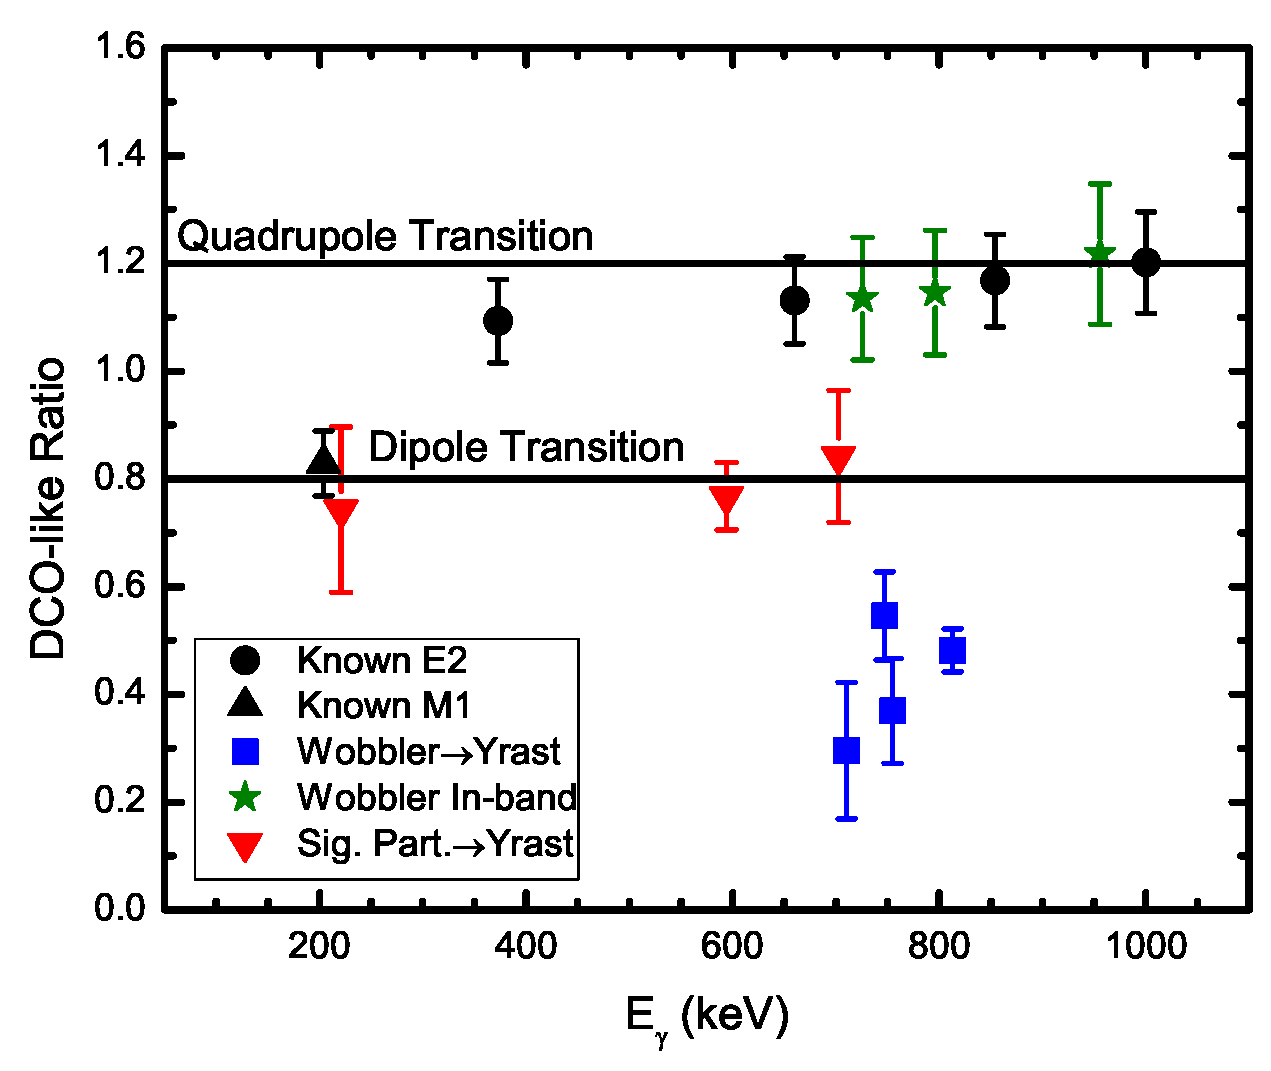
\includegraphics[width=\textwidth]{./img2/DCO.eps}}
	\caption{Schematic of heavy-ion fusion-evaporation. Adapted from }
\end{figure}

\subsection{Choice of Beam and Target}
\label{ssec:exp-pr-fus-evap-beam-target}
\subsubsection{Channel Selection}
\label{sssec:exp-pr-fus-evap-beam-target-channel}
\subsubsection{PACE4}
\label{sssec:exp-pr-fus-evap-beam-pace4}

\section{Gamma-ray Spectroscopy}
\label{sec:exp-pr-gamma-spec}
\subsection{Gamma-ray Interaction with Matter}
\label{ssec:exp-pr-gamma-spec-interactions}
\subsection{High Purity Germanium (HPGe) Detectors}
\label{ssec:exp-pr-gamma-spec-hpge}
\subsection{Escape Suppression with BGO detectors}
\label{ssec:exp-pr-gamma-spec-escape-supress}
\subsection{Gammasphere}
\label{ssec:exp-pr-gamma-gammasphere}
\subsection{Indian National Gamma Array (INGA)}
\label{ssec:exp-pr-gamma-spec-inga}

\section{Experimental Details}
\label{sec:exp-pr-details}
\subsection{ATLAS/Gammasphere}
\label{ssec:exp-pr-details-gs}
\subsection{TIFR - BARC Pelletron LINAC / INGA}
\label{ssec:exp-pr-details-inga}

\section{Data Processing}
\label{sec:exp-pr-data-proc}
\subsection{Calibration}
\label{ssec:exp-pr-data-proc-cal}
\subsection{Background Subtraction}
\label{ssec:exp-pr-data-proc-bg-sub}
\subsubsection{Symmetric Gates}
\label{sssec:exp-pr-data-proc-bg-sub-sym}
\subsubsection{Asymmetric Gates}
\label{sssec:exp-pr-data-proc-bg-sub-asym}

\section{Angular Distributions, Correlations, and Polarization}
\label{sec:exp-pr-data-ang}
\subsection{Angular Distributions}
\label{ssec:exp-pr-data-ang-dist}
Testing 1
\subsection{Angular Correlations}
\label{ssec:exp-pr-data-ang-cor}
Testing 2
\subsubsection{Directional Correlation of Gamma-rays from Oriented Nuclei DCO Ratios}
\label{sssec:exp-pr-data-ang-cor-dco}
Testing 3
\subsection{Polarization}
\label{ssec:exp-pr-data-ang-pol}
Testing 4
